\chapter{Normalising the Untyped Lambda Calculus}
\label{chap:untypednbe}

\section{Overview of the NbE algorithm}

\begin{figure}[h]
    \centering
    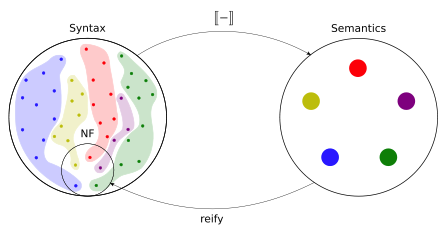
\includegraphics[width=0.6\textwidth]{./images/nbe_diagram}
    \caption{A visual overview of the NbE algorithm from \cite{slides}}
    \label{fig:nbeOverview}
\end{figure}

NbE proceeds in two steps. The first is to evaluate terms in the lambda calculus into a semantic set. In \ref{fig:nbeOverview} terms are represented by dots in the syntax set and the evaluation function is denoted by $\llbracket - \rrbracket$, which we refer to as \lstinline{eval}. The second step is to \lstinline{reify} the semantic value back into the normal form of the original term. Thus, the \lstinline{normalise} function which maps terms to their normal forms is the composition of \lstinline{eval} and \lstinline{reify}

% property of eval
\ref{fig:nbeOverview} illustrates why NbE works. The key property of the \lstinline{eval} function is that $\beta$-equal terms (represented by dots of the same colour in the syntax set) evaluate to the same semantic value. This ensures that $\beta$-equal terms normalise to the same normal form. The key property of the \lstinline{reify} function is that the codomain of \lstinline{reify} is the subset of normal forms, so \lstinline{normalise} is guaranteed to return a normal form. 

The remainer of this chapter defines the data NbE operates on and functions to perform NbE in Haskell.

\section{Syntax}

\begin{lstlisting}
    type Name = String

    data Expr = ExpVar Name
              | ExpLam Name Expr
              | ExpApp Expr Expr
\end{lstlisting}

Inhabitants of the inductively-defined datatype \lstinline{Expr} are well-formed terms of the untyped lambda calculus with strings as variables. The first argument of the lambda case introduces a new variable name bound in the function body defined by the second argument. For example, the identity function $\lambda x . x$ would be encoded as \lstinline{ExpLam "x" (ExpVar "x")}.

\begin{lstlisting}
    data NormalForm = NfNeutralForm NeutralForm
                    | NfLam Name NormalForm

    data NeutralForm = NeVar Name
                     | NeApp NeutralForm NormalForm
\end{lstlisting}

We now define the target syntax of the \lstinline{normalise} function, \lstinline{NormalForm}. Note that \lstinline{NormalForm} is inhabited by all the terms not containing $\beta$-redexes \cite{slides}, since the definition of \lstinline{NeApp} only permits application on non-lambda terms, which are encoded as values of type \lstinline{NeutralForm}.

\section{Semantics}

\begin{lstlisting}
    data V = Neutral NeutralV
           | Function (V -> V)

    data NeutralV = NeVVar Name
                  | NeVApp NeutralV V
\end{lstlisting}

% Can define V -> V in Haskell, harder in other languages, motivating advantage of Haskell?

The semantic set has a very similar structure to the set of normal forms, however lambda terms are replaced with Haskell functions of type \lstinline{V} $\rightarrow$ \lstinline{V}. The similarity simplifies \lstinline{reify} as for some terms there are obvious translations from semantics to syntax. The replacement of lambda terms will be useful in evaluating $\beta$-redexes at the semantic level instead of the syntactic level.

% Could use Neutral Form but we establish our own datatype
% Problem: fresh variables

\section{Evaluation}
To keep track of which variables have been bound by lambda terms, we introduce an environment to evaluate terms in.

\begin{lstlisting}
    type Env = Map Name V
\end{lstlisting}

Each key of the map corresponds to a bound variable name, and its associated value is the element of the semantic set representing the variable. 

\begin{lstlisting}
    eval :: Expr -> Env -> V
    eval (ExpVar x) env = case lookup x env of
            Just y -> y
            Nothing -> Neutral (NeVVar x)

    eval (ExpLam var m) env = Function f where
        f v = eval m env' where
            env' = insert var v env

    eval (ExpApp m n) env = app (eval m env) (eval n env)
\end{lstlisting}

The evaluation function takes an expression and the environment to evaluate it in, and returns the interpretation in the semantic set. 

In the variable case, we lookup the variable in the environment. If the variable was bound by an outer lambda term [WHAT IS AN OUTER LAMBDA TERM?], the variable will be present in the environment, and we can return the semantic value associated with it. Otherwise, the variables is free, so we return a semantic variable of the same name.

The semantic interpretation of a lambda expression is a Haskell function of type \lstinline{V} $\rightarrow$ \lstinline{V}. This function takes an element of the semantic set \lstinline{V}, and returns the body of the lambda evaluated in an extended environment \lstinline{env'}. In this modified environment, we introduce the variable \lstinline{var} bound by the lambda, and map this variable to . This construction is chosen as applying \lstinline{f} to an argument $v_0$ has the effect of substituting $v_0$ in place of the variable \lstinline{var} in the body of the lambda. This is similar to contracting a redex, however in NbE application of semantic elements replaces syntactic substitution.

\begin{lstlisting}
    app :: V -> V -> V
    app (Function f) v = f v
    app (Neutral n)  v = Neutral (NeVApp n v)
\end{lstlisting}


\begin{lstlisting}
    reify :: V -> FreshName NormalForm
    reify (Neutral n)  = do 
        reifiedN <- reifyNeutral n
        return (NfNeutralForm reifiedN)
    reify (Function f) = do
        freshNames <- get
        -- Remove the first name from the freshNames stream
        let freshVar = head freshNames
        -- The first name is no longer fresh (we are abount to use it as a bound variable)
        -- Modify the state to remove the used variable name
        modify tail
        -- Reify the body of the semantic function when evaluated at the fresh bound variable
        normalForm <- reify (f (Neutral (NeVVar freshVar)))
        return (NfLam freshVar normalForm)

    reifyNeutral :: NeutralV -> FreshName NeutralForm
    reifyNeutral (NeVVar i)   = return (NeVar i)
    reifyNeutral (NeVApp n m) = do
        reifiedNeutral <- reifyNeutral n
        reifiedNormal  <- reify m
        return (NeApp reifiedNeutral reifiedNormal)
\end{lstlisting}


\begin{lstlisting}
    normalise :: Expr -> NormalForm
    normalise exp = evalState (reify (eval exp empty)) freshNames 
        where
            freshNames = (getFreshVariableStream . getFreeVariables) exp
\end{lstlisting}

\section{Gensym Reification}

\subsection{Fresh variables solution 1 - Gensym}
approach based on \cite{slides}

Implemented with State monad

Issue with solution 1: Have to add monad everywhere (inescapable) - all functions dependent on state

"Less functional" - carry around state (may as well use imperative)
\section{de Bruijn Reification}
\subsection{Fresh variables solution 2 - Locally nameless terms}
approach based on \cite{deBruijn}

Uses de Bruijn Indicies for syntax and deBruijn levels for semantics

index n references nth abstraction,
if m abstractions: if n < m bound variables, otherwise free variable

Shifting for abstractions
